\section*{Estatística}
Quando falamos de média, sempre pensamos na aritmética, ou seja o somatório dos elementos dividida pela sua quantidade, que seria simplesmente o seguinte, dado o conjunto de elementos \{3, 3, 4, 6, 7\} calcular a média aritmética:

\keystroke{$3$} \keystroke{$Enter$} 
\keystroke{$3$} \keystroke{$+$} 
\keystroke{$4$} \keystroke{$+$} 
\keystroke{$6$} \keystroke{$+$} 
\keystroke{$7$} \keystroke{$+$} 
\keystroke{$5$} \keystroke{$\div$}

Que resulta em 4,60. Porém a calculadora permite realizarmos muitas outras operações estatísticas, começamos pela média geométrica:

\keystroke{$3$} \keystroke{$Enter$} 
\keystroke{$3$} \keystroke{$\times$} 
\keystroke{$4$} \keystroke{$\times$} 
\keystroke{$6$} \keystroke{$\times$} 
\keystroke{$7$} \keystroke{$\times$} 
\keystroke{$5$} \keystroke{$1/x$} \keystroke{$y^x$}

Que resulta em 4,32 ou então a média harmônica:

\keystroke{$3$} \keystroke{$1/x$} \keystroke{$+$} 
\keystroke{$3$} \keystroke{$1/x$} \keystroke{$+$} 
\keystroke{$4$} \keystroke{$1/x$} \keystroke{$+$} 
\keystroke{$6$} \keystroke{$1/x$} \keystroke{$+$} 
\keystroke{$7$} \keystroke{$1/x$} \keystroke{$+$} 
\keystroke{$5$} \keystroke{$\div$} \keystroke{$1/x$}

Que resulta em 4,08. Porém na calculadora, normalmente os dados estatísticos são armazenados como um conjunto de somas resultantes dos dados originalmente coletados. Por exemplo, para calcular a média armazenamos os dados e pressionamos a função correspondente:

Média Aritmética: 4,60 \\
\keystroke{$f$} \keystroke{$\sum$}  \keystroke{$3$} \keystroke{$\sum+$} \keystroke{$3$} \keystroke{$\sum+$} \keystroke{$4$} \keystroke{$\sum+$} \keystroke{$6$} \keystroke{$\sum+$} \keystroke{$7$} \keystroke{$\sum+$} \keystroke{$g$} \keystroke{$\bar{x}$}

Média Geométrica: 4,32 \\
\keystroke{$f$} \keystroke{$\sum$} 
\keystroke{$3$} \keystroke{$g$} \keystroke{$LN$} \keystroke{$\sum+$} 
\keystroke{$3$} \keystroke{$g$} \keystroke{$LN$} \keystroke{$\sum+$} 
\keystroke{$4$} \keystroke{$g$} \keystroke{$LN$} \keystroke{$\sum+$} 
\keystroke{$6$} \keystroke{$g$} \keystroke{$LN$} \keystroke{$\sum+$} 
\keystroke{$7$} \keystroke{$g$} \keystroke{$LN$} \keystroke{$\sum+$} 
\keystroke{$g$} \keystroke{$\bar{x}$} \keystroke{$g$} \keystroke{$e^x$}

Média Harmônica: 4,08 \\
\keystroke{$f$} \keystroke{$\sum$} 
\keystroke{$3$} \keystroke{$1/x$} \keystroke{$\sum+$} 
\keystroke{$3$} \keystroke{$1/x$} \keystroke{$\sum+$} 
\keystroke{$4$} \keystroke{$1/x$} \keystroke{$\sum+$} 
\keystroke{$6$} \keystroke{$1/x$} \keystroke{$\sum+$} 
\keystroke{$7$} \keystroke{$1/x$} \keystroke{$\sum+$} 
\keystroke{$g$} \keystroke{$\bar{x}$} \keystroke{$1/x$}

Vejamos algumas funções básicas: \vspace{-1em}
\begin{itemize}
	\item \keystroke{$f$} \keystroke{$\sum$} - Limpar os valores armazenados nos registradores
	\item \keystroke{$\sum+$} - Adicionar valores ao Somatório
	\item \keystroke{$g$} \keystroke{$\sum-$} - Subtrair valores do Somatório
	\item \keystroke{$RCL$} \keystroke{$1$} - Número de Elementos Inseridos
	\item \keystroke{$RCL$} \keystroke{$2$} - Somatório dos Elementos
	\item \keystroke{$RCL$} \keystroke{$3$} - Somatório dos Elementos ao Quadrado
\end{itemize}

\textbf{Problema 1}: O preço de venda das últimas 10 casas vendidas em um bairro distinto foi de: R\$ 198,000.00; R\$ 185.000,00; R\$ 205.200,00; R\$ 225.300,00; R\$ 206.700,00; R\$ 201.850,00; R\$ 200.000,00; R\$ 189.000,00; R\$ 192.100,00; R\$ 200.400,00. Qual é a média dos preços de venda e qual é o desvio padrão da amostra? O preço de R\$ 240.000,00 seria considerado incomum na mesma comunidade?

1. Limpar a memória: \\
\keystroke{$f$} \keystroke{$\sum$}

2. Inserir os valores (no visor cada vez que pressionamos \keystroke{$\sum+$} será mostrada a posição que o valor foi armazenado): \\
\keystroke{$1$} \keystroke{$9$} \keystroke{$8$} \keystroke{$0$} \keystroke{$0$} \keystroke{$0$} \keystroke{$\sum+$} \ \ \ \ 
\keystroke{$1$} \keystroke{$8$} \keystroke{$5$} \keystroke{$0$} \keystroke{$0$} \keystroke{$0$} \keystroke{$\sum+$} \\
\keystroke{$2$} \keystroke{$0$} \keystroke{$5$} \keystroke{$2$} \keystroke{$0$} \keystroke{$0$} \keystroke{$\sum+$} \ \ \ \ 
\keystroke{$2$} \keystroke{$2$} \keystroke{$5$} \keystroke{$3$} \keystroke{$0$} \keystroke{$0$} \keystroke{$\sum+$} \\
\keystroke{$2$} \keystroke{$0$} \keystroke{$6$} \keystroke{$7$} \keystroke{$0$} \keystroke{$0$} \keystroke{$\sum+$} \ \ \ \ 
\keystroke{$2$} \keystroke{$0$} \keystroke{$1$} \keystroke{$8$} \keystroke{$5$} \keystroke{$0$} \keystroke{$\sum+$} \\
\keystroke{$2$} \keystroke{$0$} \keystroke{$0$} \keystroke{$0$} \keystroke{$0$} \keystroke{$0$} \keystroke{$\sum+$} \ \ \ \ 
\keystroke{$1$} \keystroke{$8$} \keystroke{$9$} \keystroke{$0$} \keystroke{$0$} \keystroke{$0$} \keystroke{$\sum+$} \\
\keystroke{$1$} \keystroke{$9$} \keystroke{$2$} \keystroke{$1$} \keystroke{$0$} \keystroke{$0$} \keystroke{$\sum+$} \ \ \ \ 
\keystroke{$2$} \keystroke{$0$} \keystroke{$0$} \keystroke{$4$} \keystroke{$0$} \keystroke{$0$} \keystroke{$\sum+$}

3. Calcular a média: R\$ 200.355,00 \\
\keystroke{$g$} \keystroke{$\bar{x}$}

4. Calcular o desvio padrão: R\$ 11.189,04 \\ 
\keystroke{$g$} \keystroke{$S$}

5. Calcular os limites.

a. Limite mínimo: R\$ 177.976,91 \\
\keystroke{$g$} \keystroke{$\bar{x}$} \keystroke{$Enter$} \keystroke{$g$} \keystroke{$S$} \keystroke{$2$} \keystroke{$\times$} \keystroke{$x \lessgtr y$} \keystroke{$R \downarrow$} \keystroke{$-$}

b. Limite máximo: R\$ 222.733,09 \\
\keystroke{$x \lessgtr y$} \keystroke{$g$} \keystroke{$LSTx$} \keystroke{$+$}

No intervalo dos limites o valor de \textbf{R\$ 240.000,00} é considerado um \textit{outlier} (incomum) para esse bairro.

\textbf{Problema 2}: Um agrimensor quer saber a relação entre área construída e superfície de 8 casas localizadas em sua vizinhança. Para isso precisa conhecer a média e o desvio padrão de ambos os parâmetros. Suas medições permitiram criar a seguinte tabela:
\begin{table}[H]
	\centering 
	\begin{tabular}{R{3cm} | R{2cm} | R{3cm} | R{2cm} }
		\textbf{Superfície (em $m^2$)} & \textbf{Área (em $m^2$)} & \textbf{Superfície (em $m^2$)} & \textbf{Área (em $m^2$)} \\
		\hline
		12.000 & 3.120 & 9.000 & 2.080 \\
		10.000 & 2.560 & 10.000 & 2.700 \\
		11.000 & 2.920 & 13.000 & 3.280 \\
		14.000 & 3.300 & 12.000 & 3.080 \\
	\end{tabular}
\end{table}

1. Limpar a memória: \\
\keystroke{$f$} \keystroke{$\sum$}

2. Inserir os valores (área e superfície): \\
\keystroke{$3$} \keystroke{$1$} \keystroke{$2$} \keystroke{$0$} \keystroke{$Enter$} \keystroke{$1$} \keystroke{$2$} \keystroke{$0$} \keystroke{$0$} \keystroke{$0$} \keystroke{$\sum+$} \\
\keystroke{$2$} \keystroke{$0$} \keystroke{$8$} \keystroke{$0$} \keystroke{$Enter$} \keystroke{$9$} \keystroke{$0$} \keystroke{$0$} \keystroke{$0$} \keystroke{$0$} \keystroke{$\sum+$} \\
\keystroke{$2$} \keystroke{$5$} \keystroke{$6$} \keystroke{$0$} \keystroke{$Enter$} \keystroke{$1$} \keystroke{$0$} \keystroke{$0$} \keystroke{$0$} \keystroke{$0$} \keystroke{$\sum+$} \\
\keystroke{$2$} \keystroke{$7$} \keystroke{$0$} \keystroke{$0$} \keystroke{$Enter$} \keystroke{$1$} \keystroke{$0$} \keystroke{$0$} \keystroke{$0$} \keystroke{$0$} \keystroke{$\sum+$} \\
\keystroke{$2$} \keystroke{$9$} \keystroke{$2$} \keystroke{$0$} \keystroke{$Enter$} \keystroke{$1$} \keystroke{$1$} \keystroke{$0$} \keystroke{$0$} \keystroke{$0$} \keystroke{$\sum+$} \\
\keystroke{$3$} \keystroke{$2$} \keystroke{$8$} \keystroke{$0$} \keystroke{$Enter$} \keystroke{$1$} \keystroke{$3$} \keystroke{$0$} \keystroke{$0$} \keystroke{$0$} \keystroke{$\sum+$} \\
\keystroke{$3$} \keystroke{$3$} \keystroke{$0$} \keystroke{$0$} \keystroke{$Enter$} \keystroke{$1$} \keystroke{$4$} \keystroke{$0$} \keystroke{$0$} \keystroke{$0$} \keystroke{$\sum+$} \\
\keystroke{$3$} \keystroke{$0$} \keystroke{$8$} \keystroke{$0$} \keystroke{$Enter$} \keystroke{$1$} \keystroke{$2$} \keystroke{$0$} \keystroke{$0$} \keystroke{$0$} \keystroke{$\sum+$}

3. Média da Superfície: 11.375 $m^2$
\keystroke{$g$} \keystroke{$\bar{x}$}

4. Média da Área construída: 2.880 $m^2$ \\
\keystroke{$x \lessgtr y$}

5. Desvio Padrão da Superfície: 1.685,02 $m^2$ \\
\keystroke{$g$} \keystroke{$s$}

6. Desvio Padrão da Área construída: 415,83 $m^2$ \\
\keystroke{$x \lessgtr y$}

O desvio padrão é normalmente usado pelos investidores para medir o risco de uma ação. O desvio padrão é uma medida de volatilidade, ou seja, quanto mais os retornos da ação variarem do valor de retorno médio daquela ação, mais volátil é a ação. E conhecendo a média e o desvio padrão podemos ainda obter o \textbf{Coeficiente de Variação} que é dado pelo desvio padrão $\div$ média.

\textbf{Problema 3}: Qual empresa apresenta uma menor volatilidade pois o valor final foi exatamente o mesmo conforme os seguintes valores de abertura, variação percentual e fechamento durante a última semana:

\begin{minipage}[t]{.5\textwidth}
	\centering 
	Movimento de Ação da Empresa A
	\begin{table}[H]
		\centering 
		\begin{tabular}{R{1.3cm} | R{1cm} | R{1.3cm} }
			\textbf{Abert.} & \textbf{Var.\%} & \textbf{Fech.} \\
			\hline
			1.000,00 & 1,80 & 1.018,00 \\
			1.018,00 & 7,96 & 1.099,00 \\
			1.099,00 & 7,01 & 1.176,00 \\
			1.176,00 & -11,73 & 1.038,00 \\
			1.038,00 & 2,00 & 1.058,00 \\
		\end{tabular}
	\end{table}
\end{minipage}%
\begin{minipage}[t]{.5\textwidth}
	\centering 
	Movimento de Ação da Empresa B
	\begin{table}[H]
		\centering 
		\begin{tabular}{R{1.3cm} | R{1cm} | R{1.3cm} }
			\textbf{Abert.} & \textbf{Var.\%} & \textbf{Fech.} \\
			\hline
			1.000,00 & 6,60 & 1.066,00 \\
			1.066,00 & 12,00 & 1.194,00 \\
			1.194,00 & -9,00 & 1.086,00 \\
			1.086,00 & -4,00 & 1.043,00 \\
			1.043,00 & 1,50 & 1.058,00 \\
		\end{tabular}
	\end{table}
\end{minipage}

1. Calcular o desvio padrão para \textbf{Empresa A}: \\
\keystroke{$f$} \keystroke{$\sum$} \\
\keystroke{$1$} \keystroke{$0$} \keystroke{$0$} \keystroke{$0$} \keystroke{$\sum+$} \\
\keystroke{$1$} \keystroke{$0$} \keystroke{$1$} \keystroke{$8$} \keystroke{$\sum+$} \\ 
\keystroke{$1$} \keystroke{$0$} \keystroke{$9$} \keystroke{$9$} \keystroke{$\sum+$} \\
\keystroke{$1$} \keystroke{$1$} \keystroke{$7$} \keystroke{$6$} \keystroke{$\sum+$} \\ 
\keystroke{$1$} \keystroke{$0$} \keystroke{$3$} \keystroke{$8$} \keystroke{$\sum+$} \\ 
\keystroke{$1$} \keystroke{$0$} \keystroke{$5$} \keystroke{$8$} \keystroke{$\sum+$} \\ 
\keystroke{$g$} \keystroke{$s$}

2. Calcular o desvio padrão para \textbf{Empresa B}: \\
\keystroke{$f$} \keystroke{$\sum$} \\
\keystroke{$1$} \keystroke{$0$} \keystroke{$0$} \keystroke{$0$} \keystroke{$\sum+$} \\ 
\keystroke{$1$} \keystroke{$0$} \keystroke{$6$} \keystroke{$6$} \keystroke{$\sum+$} \\
\keystroke{$1$} \keystroke{$1$} \keystroke{$9$} \keystroke{$4$} \keystroke{$\sum+$} \\
\keystroke{$1$} \keystroke{$0$} \keystroke{$8$} \keystroke{$6$} \keystroke{$\sum+$} \\
\keystroke{$1$} \keystroke{$0$} \keystroke{$4$} \keystroke{$3$} \keystroke{$\sum+$} \\
\keystroke{$1$} \keystroke{$0$} \keystroke{$5$} \keystroke{$8$} \keystroke{$\sum+$} \\
\keystroke{$g$} \keystroke{$s$}

A ação da Empresa A apresenta um desvio padrão de \textbf{R\$ 64,33} enquanto que a ação da Empresa B é de \textbf{R\$ 65,27} sendo esta a mais volátil.

\textbf{Erro Padrão} é uma medida de quão confiável é a média de uma amostra como um estimador da média de uma população na qual a amostra foi retirada.

\textbf{Problema 4}: Uma amostra com 6 aluguéis para apartamentos de um quarto demonstrou o seguinte resultado: R\$ 190,00; R\$ 200,00; dois aluguéis R\$ 205,00; R\$ 216,00; R\$ 220,00. Qual média, desvio e erro padrão?

1. Entrada dos dados: \\
\keystroke{$f$} \keystroke{$REG$} \\
\keystroke{$1$} \keystroke{$9$} \keystroke{$0$} \keystroke{$\sum+$} \\ 
\keystroke{$2$} \keystroke{$0$} \keystroke{$0$} \keystroke{$\sum+$} \\ 
\keystroke{$2$} \keystroke{$0$} \keystroke{$5$} \keystroke{$\sum+$} \\ 
\keystroke{$2$} \keystroke{$0$} \keystroke{$5$} \keystroke{$\sum+$} \\ 
\keystroke{$2$} \keystroke{$1$} \keystroke{$6$} \keystroke{$\sum+$} \\ 
\keystroke{$2$} \keystroke{$2$} \keystroke{$0$} \keystroke{$\sum+$}

2. Média: R\$ 206,00 \\
\keystroke{$g$} \keystroke{$\bar{x}$}

3. Desvio padrão: R\$ 10,86 \\
\keystroke{$g$} \keystroke{$S$}

4. Erro padrão: R\$ 4,43 \\
\keystroke{$RCL$} \keystroke{$1$} \keystroke{$g$} \keystroke{$\sqrt{x}$}  \keystroke{$\div$}

\textbf{Problema 5}: Uma pesquisa registrou o valor dos aluguéis para apartamentos de um quarto: 54 por R\$ 190,00; 32 por R\$ 195,00; 88 por R\$ 200,00; 92 por R\$ 206,00. Qual média, desvio e erro padrão?

1. Entrada dos dados: \\
\keystroke{$f$} \keystroke{$REG$} \\
\keystroke{$1$} \keystroke{$9$} \keystroke{$0$} \keystroke{$Enter$} 
\keystroke{$Enter$} \keystroke{$5$} \keystroke{$4$} \keystroke{$STO$}
\keystroke{$+$} \keystroke{$0$} \keystroke{$\times$} \keystroke{$\sum+$} \\ 
\keystroke{$1$} \keystroke{$9$} \keystroke{$5$} \keystroke{$Enter$} 
\keystroke{$Enter$} \keystroke{$3$} \keystroke{$2$} \keystroke{$STO$}
\keystroke{$+$} \keystroke{$0$} \keystroke{$\times$} \keystroke{$\sum+$} \\ 
\keystroke{$2$} \keystroke{$0$} \keystroke{$0$} \keystroke{$Enter$} 
\keystroke{$Enter$} \keystroke{$8$} \keystroke{$8$} \keystroke{$STO$}
\keystroke{$+$} \keystroke{$0$} \keystroke{$\times$} \keystroke{$\sum+$} \\ 
\keystroke{$2$} \keystroke{$0$} \keystroke{$6$} \keystroke{$Enter$} 
\keystroke{$Enter$} \keystroke{$9$} \keystroke{$2$} \keystroke{$STO$}
\keystroke{$+$} \keystroke{$0$} \keystroke{$\times$} \keystroke{$\sum+$} \\ 

2. Média mensal: R\$ 199,44 \\
\keystroke{$RCL$} \keystroke{$0$} \keystroke{$STO$} \keystroke{$1$} \keystroke{$RCL$} \keystroke{$6$} \keystroke{$STO$} \keystroke{$3$} \keystroke{$g$} \keystroke{$\bar{x}$}

3. Desvio padrão: R\$ 5,97 \\
\keystroke{$g$} \keystroke{$S$}

4. Erro padrão: R\$ 0,37 \\
\keystroke{$RCL$} \keystroke{$1$} \keystroke{$g$} \keystroke{$\sqrt{x}$}  \keystroke{$\div$}

\subsection*{Covariância}
É uma medida da interdependência entre variáveis emparelhadas (x e y). Como o desvio padrão, a covariância pode ser definida para uma amostra ($S_{xy}$) ou uma população ($S'_{xy}$) da seguinte forma: \vspace{-1em}
\begin{itemize} 
	\item $S_{xy} = r \times sx \times sy$
	\item $S'_{xy} = r \times s'x \times s'y$
\end{itemize} 

\textbf{Problema 1}: Encontrar a covariância da amostra e da população para as seguintes variáveis emparelhadas:
\begin{table}[H]
	\centering 
	\begin{tabular}{l | r | r | r | r | r | r | r }
		$x_i$ & 26 & 30 & 44 & 50 & 62 & 68 & 74 \\
		$y_i$ & 92 & 85 & 78 & 81 & 54 & 51 & 40 \\
	\end{tabular}
\end{table}

1. Entrada dos dados: \\
\keystroke{$f$} \keystroke{$REG$} \\
\keystroke{$9$} \keystroke{$2$} \keystroke{$Enter$} \keystroke{$2$} \keystroke{$6$} \keystroke{$\sum+$} \\
\keystroke{$8$} \keystroke{$5$} \keystroke{$Enter$} \keystroke{$3$} \keystroke{$0$} \keystroke{$\sum+$} \\
\keystroke{$7$} \keystroke{$8$} \keystroke{$Enter$} \keystroke{$4$} \keystroke{$4$} \keystroke{$\sum+$} \\
\keystroke{$8$} \keystroke{$1$} \keystroke{$Enter$} \keystroke{$5$} \keystroke{$0$} \keystroke{$\sum+$} \\
\keystroke{$5$} \keystroke{$4$} \keystroke{$Enter$} \keystroke{$6$} \keystroke{$2$} \keystroke{$\sum+$} \\
\keystroke{$5$} \keystroke{$1$} \keystroke{$Enter$} \keystroke{$6$} \keystroke{$8$} \keystroke{$\sum+$} \\
\keystroke{$4$} \keystroke{$0$} \keystroke{$Enter$} \keystroke{$7$} \keystroke{$4$} \keystroke{$\sum+$}

2. Covariância da amostra: -354,14 \\
\keystroke{$g$} \keystroke{$s$} \keystroke{$\times$} \keystroke{$Enter$} \keystroke{$g$} \keystroke{$\hat{y},r$} \keystroke{$R \downarrow$} \keystroke{$\times$}

3. Covariância da população: -303,55 \\
\keystroke{$RCL$} \keystroke{$1$} \keystroke{$1$} \keystroke{$-$} \keystroke{$RCL$} \keystroke{$1$} \keystroke{$\div$} \keystroke{$\times$}

\subsection*{Ajuste de curva exponencial}
Para quadrados mínimos pode ser calculado de acordo com a equação $y = Ae^{Bx}$. A técnica para o ajuste de curva exponencial é utilizado para determinar a taxa de crescimento com uma variável como o valor de uma ação ao longo do tempo, quando há suspeita de que o desempenho é não linear. Onde o valor de \textbf{B} é o valor decimal da taxa de crescimento contínuo. 

Por exemplo, após digitar várias cotações de preços para o fim de mês a uma determinada ação, o valor de B é 0,10. Isso significa que, durante este período medido o estoque experimentou uma taxa de crescimento contínuo de 10\%. Se B for maior que 0, teremos uma curva de crescimento.

\textbf{Problema 1}: O preço histórico de uma ação foi registrado conforme a seguinte disposição: 2001 - R\$ 45,00; 2002 - R\$ 51,00; 2002 - R\$ 53,00; 2003 - R\$ 72,00; 2004 - R\$ 85,00; 2005 - R\$ 97,00. Qual a Taxa efetiva de crescimento e se continuar qual será o preço projetado ao final de 2006 (ano 7)?

1. Entrada dos dados: \\
\keystroke{$f$} \keystroke{$REG$} \\
\keystroke{$4$} \keystroke{$5$} \keystroke{$g$} \keystroke{$LN$} \keystroke{$1$} \keystroke{$\sum+$} \\
\keystroke{$5$} \keystroke{$1$} \keystroke{$g$} \keystroke{$LN$} \keystroke{$2$} \keystroke{$\sum+$} \\
\keystroke{$5$} \keystroke{$3$} \keystroke{$g$} \keystroke{$LN$} \keystroke{$3$} \keystroke{$\sum+$} \\
\keystroke{$7$} \keystroke{$2$} \keystroke{$g$} \keystroke{$LN$} \keystroke{$4$} \keystroke{$\sum+$} \\
\keystroke{$8$} \keystroke{$5$} \keystroke{$g$} \keystroke{$LN$} \keystroke{$5$} \keystroke{$\sum+$} \\
\keystroke{$9$} \keystroke{$7$} \keystroke{$g$} \keystroke{$LN$} \keystroke{$6$} \keystroke{$\sum+$}

2. Coeficiente de correlação (entre y e x): 0,98 \\
\keystroke{$g$} \keystroke{$\hat{y},r$} \keystroke{$x \lessgtr y$}

3. Valor de \textbf{A}: 36,57 \\
\keystroke{$0$} \keystroke{$g$} \keystroke{$\hat{y},r$} \keystroke{$g$} \keystroke{$e^x$} 

4. Valor de \textbf{B}: 0,16 \\
\keystroke{$1$} \keystroke{$g$} \keystroke{$\hat{y},r$} \keystroke{$g$} \keystroke{$e^x$} \keystroke{$0$} \keystroke{$g$} \keystroke{$\hat{y},r$} \keystroke{$g$} \keystroke{$e^x$} \keystroke{$x \lessgtr y$} \keystroke{$R \downarrow$} \keystroke{$\div$} \keystroke{$g$} \keystroke{$LN$}

5. Taxa efetiva de crescimento: 0,18 \\
\keystroke{$g$} \keystroke{$e^x$} \keystroke{$1$} \keystroke{$-$} 

6. Projeção do preço para 2006: R\$ 113,87 \\
\keystroke{$7$} \keystroke{$g$} \keystroke{$\hat{y},r$} \keystroke{$g$} \keystroke{$e^x$} 

\textbf{Problema 2}: Um fabricante observou as vendas de um produto ao longo de vários meses, foi registrado os seguintes valores: 1431; 3506; 5177; 6658; 7810; 8592. Estes podem ser ajustados por uma curva logarítmica da forma $y = A + B (ln\ x)$, onde $y$ representa as vendas cumulativas em unidades e $x$ o número de meses desde o início. Quantas unidades serão vendidas ao final do sétimo e oitavo mês?

1. Entrada dos dados: \\
\keystroke{$f$} \keystroke{$REG$} \\
\keystroke{$1$} \keystroke{$4$} \keystroke{$3$} \keystroke{$1$} \keystroke{$Enter$} \keystroke{$1$}  \keystroke{$g$} \keystroke{$LN$} \keystroke{$\sum+$} \\
\keystroke{$3$} \keystroke{$5$} \keystroke{$0$} \keystroke{$6$} \keystroke{$Enter$} \keystroke{$2$}  \keystroke{$g$} \keystroke{$LN$} \keystroke{$\sum+$} \\
\keystroke{$5$} \keystroke{$1$} \keystroke{$7$} \keystroke{$7$} \keystroke{$Enter$} \keystroke{$3$}  \keystroke{$g$} \keystroke{$LN$} \keystroke{$\sum+$} \\
\keystroke{$6$} \keystroke{$6$} \keystroke{$5$} \keystroke{$8$} \keystroke{$Enter$} \keystroke{$4$}  \keystroke{$g$} \keystroke{$LN$} \keystroke{$\sum+$} \\
\keystroke{$7$} \keystroke{$8$} \keystroke{$1$} \keystroke{$0$} \keystroke{$Enter$} \keystroke{$5$}  \keystroke{$g$} \keystroke{$LN$} \keystroke{$\sum+$} \\
\keystroke{$8$} \keystroke{$5$} \keystroke{$9$} \keystroke{$2$} \keystroke{$Enter$} \keystroke{$6$}  \keystroke{$g$} \keystroke{$LN$} \keystroke{$\sum+$}

2. Coeficiente de correlação (entre y e x): 0,99 \\
\keystroke{$g$} \keystroke{$\hat{y},r$} \keystroke{$x \lessgtr y$}

3. Valor de \textbf{A}: 1.066,15 \\
 \keystroke{$0$} \keystroke{$g$} \keystroke{$\hat{y},r$} 

4. Valor de \textbf{B}: 4.069,93 \\
\keystroke{$1$} \keystroke{$g$} \keystroke{$\hat{y},r$} \keystroke{$Enter$} \keystroke{$0$} \keystroke{$g$} \keystroke{$\hat{y},r$} \keystroke{$x \lessgtr y$} \keystroke{$R \downarrow$} \keystroke{$-$}

5. Projeção de vendas para o sétimo mês: 8.985,87 unidades \\
\keystroke{$7$} \keystroke{$g$} \keystroke{$LN$} \keystroke{$g$} \keystroke{$\hat{y},r$} 

6. Projeção de vendas para o oitavo mês: 9.529,34 unidades \\
\keystroke{$8$} \keystroke{$g$} \keystroke{$LN$} \keystroke{$g$} \keystroke{$\hat{y},r$} 

\textbf{Problema 3}: Ao investigar quantitativamente a relação entre o tempo (t) para um objeto em queda atingir o solo e a altura (h) em que caiu, foi lançado uma pedra de vários níveis e cronometrado sua descida resultando nas seguintes medidas: t = 2 e h = 30; t = 2,5 e h = 50; t = 3,5 e h = 90; t = 4 e h = 130; t = 4.5 e h = 150. Encontre a fórmula da curva de potência que melhor expressa h como uma função de t ($h = A \times t^B$).

1. Entrada dos dados: \\
\keystroke{$f$} \keystroke{$REG$} \\
\keystroke{$3$} \keystroke{$0$} \keystroke{$g$} \keystroke{$LN$}
\keystroke{$2$} \keystroke{$g$} \keystroke{$LN$} \keystroke{$\sum+$} \\
\keystroke{$5$} \keystroke{$0$} \keystroke{$g$} \keystroke{$LN$}
\keystroke{$2$} \keystroke{$.$} \keystroke{$5$} \keystroke{$g$} \keystroke{$LN$} \keystroke{$\sum+$} \\
\keystroke{$9$} \keystroke{$0$} \keystroke{$g$} \keystroke{$LN$}
\keystroke{$3$} \keystroke{$.$} \keystroke{$5$} \keystroke{$g$} \keystroke{$LN$} \keystroke{$\sum+$} \\
\keystroke{$1$} \keystroke{$3$} \keystroke{$0$} \keystroke{$g$} \keystroke{$LN$}
\keystroke{$4$} \keystroke{$g$} \keystroke{$LN$} \keystroke{$\sum+$} \\
\keystroke{$1$} \keystroke{$5$} \keystroke{$0$} \keystroke{$g$} \keystroke{$LN$} 
\keystroke{$4$} \keystroke{$.$} \keystroke{$5$} \keystroke{$g$} \keystroke{$LN$} \keystroke{$\sum+$}

2. Coeficiente de correlação (entre y e x): 1,0 \\
\keystroke{$g$} \keystroke{$\hat{y},r$} \keystroke{$x \lessgtr y$}

3. Valor de \textbf{A}: 7,72 \\
\keystroke{$0$} \keystroke{$g$} \keystroke{$\hat{y},r$} \keystroke{$g$} \keystroke{$e^x$}

4. Valor de \textbf{B}: 1,99 \\
\keystroke{$1$} \keystroke{$g$} \keystroke{$\hat{y},r$} \keystroke{$Enter$} \keystroke{$0$} \keystroke{$g$} \keystroke{$\hat{y},r$} 
\keystroke{$x \lessgtr y$} \keystroke{$R \downarrow$} \keystroke{$-$}

A fórmula que melhor expressa é: $h = 7,72 \times t^{1,99}$

\subsection*{Qui-quadrado}
Esta é uma medida da qualidade do ajuste entre dois conjuntos de frequências. É usado para testar se um conjunto de observações difere de outro com frequências esperadas o suficiente para rejeitar a hipótese de quais frequências esperadas foram obtidas.

\textbf{Problema 1}: Um dado suspeito de um cassino em Las Vegas foi levado a uma empresa de testes para determinar sua honestidade. O dado é lançado 120 vezes e os seguintes resultados foram obtidos: 1 - 25; 2 - 17; 3 - 15; 4 - 23; 5 - 24; 6 - 16. A frequência esperada era 20 para cada número (120 lançamentos $\div$ 6 lados).

1. Preparação para os dados: \\
\keystroke{$f$} \keystroke{$REG$} \\
\keystroke{$2$} \keystroke{$0$} \keystroke{$STO$} \keystroke{$0$}

2. Para face 1: 1,25 \\
\keystroke{$2$} \keystroke{$5$} \keystroke{$Enter$} \keystroke{$RCL$} \keystroke{$0$} \keystroke{$-$} \keystroke{$Enter$} \keystroke{$\times$} \keystroke{$RCL$} \keystroke{$0$} \keystroke{$\div$}

2. Para face 2: 0,45 - Acumulado 1,70 \\
\keystroke{$1$} \keystroke{$7$} \keystroke{$Enter$} \keystroke{$RCL$} \keystroke{$0$} \keystroke{$-$} \keystroke{$Enter$} \keystroke{$\times$} \keystroke{$RCL$} \keystroke{$0$} \keystroke{$\div$} \keystroke{$+$}

2. Para face 3: 1,25 - Acumulado 2,95 \\
\keystroke{$1$} \keystroke{$5$} \keystroke{$Enter$} \keystroke{$RCL$} \keystroke{$0$} \keystroke{$-$} \keystroke{$Enter$} \keystroke{$\times$} \keystroke{$RCL$} \keystroke{$0$} \keystroke{$\div$} \keystroke{$+$}

2. Para face 4: 0,45 - Acumulado 3,40 \\
\keystroke{$2$} \keystroke{$3$} \keystroke{$Enter$} \keystroke{$RCL$} \keystroke{$0$} \keystroke{$-$} \keystroke{$Enter$} \keystroke{$\times$} \keystroke{$RCL$} \keystroke{$0$} \keystroke{$\div$} \keystroke{$+$}

2. Para face 5: 0,80 - Acumulado 4,20 \\
\keystroke{$2$} \keystroke{$4$} \keystroke{$Enter$} \keystroke{$RCL$} \keystroke{$0$} \keystroke{$-$} \keystroke{$Enter$} \keystroke{$\times$} \keystroke{$RCL$} \keystroke{$0$} \keystroke{$\div$} \keystroke{$+$}

2. Para face 6: 0,80 - Acumulado 5,00 \\
\keystroke{$1$} \keystroke{$6$} \keystroke{$Enter$} \keystroke{$RCL$} \keystroke{$0$} \keystroke{$-$} \keystroke{$Enter$} \keystroke{$\times$} \keystroke{$RCL$} \keystroke{$0$} \keystroke{$\div$} \keystroke{$+$}

O número com graus de liberdade é $n - 1$, sendo 6 possibilidades, temos o valor \textbf{5} (5 graus de liberdade ou probabilidade = 0,95). Ao consultar a tabela Qui-quadrado ao final desta apostila, observamos $x^2$ e nível com significância de 0,05 e igual a \textbf{11,07}. Como o acumulado é um valor menor concluímos que o dado é justo.

\subsection*{Regressão}
Na HP-12C, somatórios resultantes de dados estatísticos são apropriados cálculos de regressão linear. Os valores de um gráfico devem ser entrados para se calcular a equação da linha, obedecendo a sequencia: ordenada e abcissa. 

\textbf{Problema 1}: Calcular a inclinação para caracterizar a linha reta e da abcissa (x) quando a ordenada (y) for igual a 8, com base na informação do seguinte gráfico:
\begin{figure}[H]
	\centering
	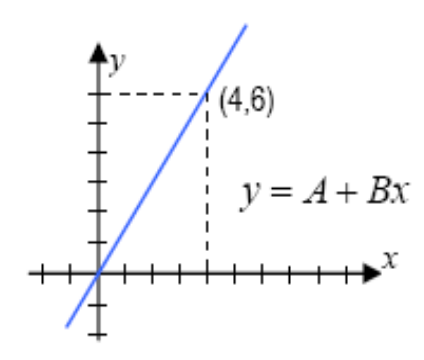
\includegraphics[width=0.35\textwidth]{images/reta01}
	\caption{Exemplo 01}
\end{figure}

1. Limpar a memória: \keystroke{$f$} \keystroke{$\sum$}

2. Entrar com os valores: \keystroke{$0$} \keystroke{$Enter$} \keystroke{$0$} \keystroke{$\sum+$} \keystroke{$6$} \keystroke{$Enter$} \keystroke{$4$} \keystroke{$\sum+$}

3. Calcular a inclinação: \keystroke{$1$} \keystroke{$g$} \keystroke{$\hat{y},r$}

4. Calcular o valor da ordenada: \keystroke{$8$} \keystroke{$g$} \keystroke{$\hat{y},r$} 

E assim temos uma inclinação de \textbf{1,50} e para abcissa com valor 8 a ordenada é igual a \textbf{12}.

\textbf{Problema 2}: Calcular o ponto de interceptação-y, a inclinação para caracterizar a linha reta e o valor da abcissa quando a ordenada for igual a 5 com base na informação do seguinte gráfico:
\begin{figure}[H]
	\centering
	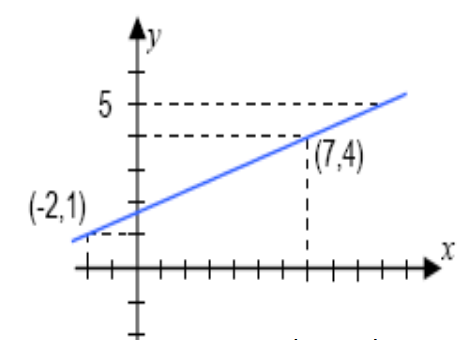
\includegraphics[width=0.35\textwidth]{images/reta02}
	\caption{Exemplo 02}
\end{figure}

1. Limpar a memória: \\
\keystroke{$f$} \keystroke{$\sum$}

2. Entrar com os valores: \\
\keystroke{$1$} \keystroke{$Enter$} \keystroke{$2$} \keystroke{$CHS$} \keystroke{$\sum+$} \keystroke{$4$} \keystroke{$Enter$} \keystroke{$7$} \keystroke{$\sum+$}

3. Calcular a interceptação-y (A): 1,67 \\
\keystroke{$0$} \keystroke{$g$} \keystroke{$\hat{y},r$}

4. Calcular a inclinação (B): 0,33 \\
\keystroke{$1$} \keystroke{$g$} \keystroke{$\hat{y},r$} \keystroke{$x \lessgtr y$} \keystroke{$R \downarrow$} \keystroke{$x \lessgtr y$} \keystroke{$-$}

5. Calcular o valor da abcissa: 10 \\
\keystroke{$5$} \keystroke{$g$} \keystroke{$\hat{x},r$} 

\textbf{Problema 3}: Estimar as vendas previstas de uma fábrica para o ano de 2019 e em que ano as vendas chegam a 130.000 unidades conforme o seguinte detalhamento (as vendas estão em mil unidades): 2010 - 58; 2011 - 66; 2012 - 72; 2013 - 77; 2014 - 81; 2015 - 85.

Uma forma de estimar o comportamento das vendas futuras consiste em aplicar o Método dos Mínimos Quadrados, que permite encontrar a melhor reta que se ajusta aos pontos.

1. Limpar a memória: \\
\keystroke{$f$} \keystroke{$\sum$}

2. Entrar com os valores (para agilizar a digitação podemos usar o ano com 2 dígitos): \\
\keystroke{$5$} \keystroke{$8$} \keystroke{$Enter$} \keystroke{$1$} \keystroke{$0$} \keystroke{$\sum+$} \\
\keystroke{$6$} \keystroke{$6$} \keystroke{$Enter$} \keystroke{$1$} \keystroke{$1$} \keystroke{$\sum+$} \\
\keystroke{$7$} \keystroke{$2$} \keystroke{$Enter$} \keystroke{$1$} \keystroke{$2$} \keystroke{$\sum+$} \\
\keystroke{$7$} \keystroke{$7$} \keystroke{$Enter$} \keystroke{$1$} \keystroke{$3$} \keystroke{$\sum+$} \\
\keystroke{$8$} \keystroke{$1$} \keystroke{$Enter$} \keystroke{$1$} \keystroke{$4$} \keystroke{$\sum+$} \\
\keystroke{$8$} \keystroke{$5$} \keystroke{$Enter$} \keystroke{$1$} \keystroke{$5$} \keystroke{$\sum+$} 

3. Vendas previstas para o ano de 2019: 107,52 mil unidades \\ 
\keystroke{$1$} \keystroke{$9$} \keystroke{$g$} \keystroke{$\hat{y},r$}

4. Ano para 130.000 unidades: 2023 \\
\keystroke{$1$} \keystroke{$3$} \keystroke{$0$} \keystroke{$g$} \keystroke{$\hat{x},r$}

\subsection*{Programação com Permutação e Combinação}
Programar na HP-12C consiste em gravar uma sequência de teclas, este é um recurso muito útil para determinadas situações. É possível inserir no máximo 99 linhas na memória. As principais teclas a saber são: \vspace{-1em}
\begin{itemize}
	\item \keystroke{$R/S$} \textit{RUN/STOP}, iniciar ou interromper a execução de um programa
	\item \keystroke{$f$} \keystroke{$P/R$} \textit{PROGRAM/RUN}, colocar a calculadora em modo de programação ou execução
	\item \keystroke{$g$} \keystroke{$PSE$} \textit{PAUSE}, fornecer uma pausa com cerca de 1 seg. na execução do programa
	\item \keystroke{$f$} \keystroke{$PRGM$} \textit{CLEAR PROGRAMS}, limpar os programas registrados na memória da calculadora
	\item \keystroke{$g$} \keystroke{$GTO$} \textit{GO TO}, executar um desvio de rotina no programa
	\item \keystroke{$g$} \keystroke{$BST$} \textit{STEP}, executar o programa passo a passo
\end{itemize}

\textbf{Permutação} (também chamada de Arranjo Simples) é um subconjunto ordenado em um conjunto de objetos distintos. O número de permutações possíveis, cada uma contendo n objetos, que podem ser formadas a partir de m objetos distintos é dado por: $_mP_n = m! \div (m - n)!$ Lembre-se que na permutação não existe repetição e o número de elementos a serem tomados para compor o resultado deve ser igual ao número de elementos no conjunto.

Por exemplo, seja T um conjunto com elementos: \{A,B,C,D\}, e queremos realizar agrupamentos com 2 elementos quantos arranjos podemos obter. Para resolvermos na calculadora criamos o seguinte programa:

\keystroke{$f$} \keystroke{$P/R$} \\
\keystroke{$f$} \keystroke{$PRGM$} - 00 \\
\keystroke{$STO$} \keystroke{$0$} - 01 \\
\keystroke{$x \lessgtr y$} - 02 \\
\keystroke{$g$} \keystroke{$n!$} - 03 \\
\keystroke{$g$} \keystroke{$LST x$} - 04 \\
\keystroke{$RCL$} \keystroke{$0$} - 05 \\
\keystroke{$-$} - 06 \\
\keystroke{$g$} \keystroke{$n!$} - 07 \\
\keystroke{$\div$} - 08 \\
\keystroke{$g$} \keystroke{$GTO$} \keystroke{$0$} \keystroke{$0$} - 09 \\
\keystroke{$f$} \keystroke{$P/R$}

E para executar o programa: \keystroke{$4$} \keystroke{$Enter$} \keystroke{$2$} \keystroke{$R/S$} e temos como resposta 12. Ou seja: \\
$_4P_2$ = \{AB, AC, AD, BA, BC, BD, CA, CB, CD, DA, DB, DC\}

\textbf{Problema 1}: De quantas maneiras diferentes 10 pessoas podem sentar em um banco se só existem 4 lugares disponíveis? ($_{10}P_4$)

\keystroke{$1$} \keystroke{$0$} \keystroke{$Enter$} \keystroke{$4$} \keystroke{$R/S$}

E temos 5.040 maneiras diferentes.

\textbf{Problema 2}: Uma corrida com 20 atletas vai premiar os 5 primeiros, quantos arranjos são possíveis realizar? ($_{20}P_5$)

\keystroke{$2$} \keystroke{$0$} \keystroke{$Enter$} \keystroke{$5$} \keystroke{$R/S$}

E temos 1.860.480 maneiras diferentes.

\textbf{Combinação} é uma seleção com um ou mais conjuntos de objetos distintos, independentemente da ordem. O número de combinações possíveis, cada uma contendo n objetos, que podem ser formadas a partir de uma coleção de m objetos distintos é dado por: $_mC_n = m! \div (m - n)!n!$

Por exemplo, seja T um conjunto com elementos: \{A,B,C,D\}, e queremos realizar agrupamentos com 2 elementos quantos arranjos podemos obter sem a repetição desses. Para resolvermos na calculadora criamos o seguinte programa:

\keystroke{$f$} \keystroke{$P/R$} \\
\keystroke{$f$} \keystroke{$PRGM$} - 00 \\
\keystroke{$STO$} \keystroke{$0$} - 01 \\
\keystroke{$x \lessgtr y$} - 02 \\
\keystroke{$g$} \keystroke{$n!$} - 03 \\
\keystroke{$g$} \keystroke{$LST x$} - 04 \\
\keystroke{$RCL$} \keystroke{$0$} - 05 \\
\keystroke{$-$} - 06 \\
\keystroke{$g$} \keystroke{$n!$} - 07 \\
\keystroke{$RCL$} \keystroke{$0$} - 08 \\
\keystroke{$g$} \keystroke{$n!$} - 09 \\
\keystroke{$\times$} - 10 \\
\keystroke{$\div$} - 11 \\
\keystroke{$g$} \keystroke{$GTO$} \keystroke{$0$} \keystroke{$0$} - 12 \\
\keystroke{$f$} \keystroke{$P/R$}

E para executar o programa: \keystroke{$4$} \keystroke{$Enter$} \keystroke{$2$} \keystroke{$R/S$} e temos como resposta 6. Ou seja: \\
$_4C_2$ = \{AB ou BA, AC ou CA, AD ou DA, BC ou CB, BD ou DB, CD ou DC\}

\textbf{Problema 1}: Um coordenador precisa selecionar um comitê formado por três pessoas entre os sete engenheiros que trabalham para ele. De quantas maneiras diferentes o comitê pode ser selecionado? $_7C_3$

\keystroke{$7$} \keystroke{$Enter$} \keystroke{$3$} \keystroke{$R/S$}

E temos 35 maneiras diferentes.

\textbf{Problema 2}: A megassena consiste em uma cartela de 60 números dentre os quais devemos acertar 6 para ganharmos o prêmio principal, quantas possibilidades existem? $_60C_6$

\keystroke{$6$} \keystroke{$0$} \keystroke{$Enter$} \keystroke{$6$} \keystroke{$R/S$}

E temos 50.063.860 maneiras diferentes.




